\documentclass[twocolumn]{article}
\usepackage{ml_homework_template}
\usepackage{amsmath,amsthm,amssymb}
\usepackage[pdftex]{graphicx}

% You should submit your final project by emailing it to fp@class.brml.org. The subject line must read "final project". 
% If the subject line does not match, an error email is returned; otherwise, a positive ACK is replied. Automated deadline 
% checking is implemented. The submission must be in before Feb. 8, 2014 (i.e., by Feb, 7, 23:59 CET). Please submit the 
% following:
%•	a short "paper" describing what you did, describing the data, describing the method, and your results. Please keep 
%   it succinct, with the class teachers as readership in mind. It should contain plots describing your results. This 
%   paper must be submitted in PDF format.
%•	all software necessary to reproduce your results, i.e., also the methodologies to preprocess the data.

\title{Final Project of Machine Learning\\-\\Forests and Ferests}


\author{
\name{Jonas Uhrig}\\
\imat{03616049}\\
\email{jonas.uhrig@in.tum.de}
\And
\name{Michael Wolfram} \\
\imat{03616011}\\
\email{michaelwolfram@gmx.de}
}



\begin{document}
\onecolumn
\maketitle

\section*{Abstract}

In this paper we describe our final project for the Machine Learning class of 2013/14 at TUM. We use data set 4) containing information about body postures and movements and apply two similar Machine Learning algorithms that were implemented within this project. The used algorithms are called 'Ferns' and 'Binary Tree' or 'Random Forest' - we also cover different variations of those algorithms. Moreover, we applied heuristical approaches used for Trees to our Ferns to evaluate advantages regarding classification accuracy.\\
The programming language of our choice is Matlab - some of the used approaches on Ferns are based on ideas from Mustafa \"Ozuyal et al. [1], the development of the trees and forests was only based on ideas from the lecture.



\twocolumn

\section{Approach}
% 'what you did'
We already know about Trees and Forests from the lecture - additionally we read of a Machine Learning algorithm called \textit{Ferns} [1], which was recently (2007) introduced to detect objects or keypoints in images. Ferns have a very similar behaviour as Forests and, in fact, are completely replaceable - though the important difference lies in the striking speed for training a Fern. This is the case because a Fern has only $n$ nodes where a Tree has $2^n$ nodes. A Tree can be transformed into a Fern by applying the same tests in every node of a Tree-layer and then 'shrinking' it horizontally to consist of only one node per layer.

For object detection purposes, Ferns are built using binary values as feature vector which initially posed a problem for the chosen PUC-Rio data set containing continuous (e.g the sensor data) and categorical (e.g gender, names) features. A key point of Ferns is chance so we thought it might serve to randomly choose a threshold within the range of each feature and do a simple comparison, resulting in a new binary feature value - this approach was also used by Kursa [2], which encouraged us to continue the implementation.

The goal of this project is, besides the implementation of the two chosen algorithms, the evaluation of Ferns on data with non-binary attributes. Within the original application area of Ferns (fast keypoint recognition), Ferns outperform Trees. Thus, we wanted to evaluate if this relation also holds true for the given data set. To achieve this, we applied various available methods to optimize the classification accuracy of our algorithms in order to compare Ferns and Trees in full depth.


\section{Data}
sitting: 50631
sittingdown: 11827
standing: 47370
standingup: 12415
walking: 43390



\section{Method}
This section gives a short overview of the properties of both methods. The algorithms and basic methods to optimize them were taken from the original papers (see section ''References'') and some lecture slides. In the final implementation we made some slight changes to cope with the given restrictions of this project.

\subsection{Forest}

\subsubsection{Basic Principle}
As known from the lecture, we implemented a Forest as ensemble of a certain number of Decision Trees. Our Trees are defined by the following parameters:\\
We implemented bagging and feature subset selection for the training of each Tree of a Forest to overcome overfitting on the whole data set. When using bagging, the data set that a single Tree may use for its training phase is randomly drawn from the original training set of the Forest with replacement. Therefore, pruning as third method became superfluous. The random selection of feature subsets induces a parameter to the Tree: the number $d<D$ of features, with $D$ being the total number of features, which is used for finding best splits in each node of the Tree.\\
Other properties of a Tree are its criteria when to stop growing. We implemented the four suggestions from the lecture: The depth of the tree can be limited to a certain maximum. A lower bound for the benefit of another split can be specified. If the number of training samples in a certain node is below a given threshold it will not be split any more and is marked as leaf and lastly, the tree stops growing at a particular node if the distribution of labels/classes of the training data in this node is pure.\\
For the last stopping heuristic we implemented the impurity measures \textit{Gini index}, \textit{Entropy} and \textit{misclassification rate} as stated in the lecture. After some small initial tests we decided to concentrate on the \textit{Gini index} for further testing since it was more accurate on a subset of the given training data even though the \textit{Entropy} was slightly faster.\\
We used the same settings for each Tree of a Forest.

\subsubsection{Optimizations}
Due to the fact that we were faced with limitations regarding time and computation power we did minor modifications to the building process of a Forest. Rather than building a whole new Forest for each different number of Trees within the Forest we just added a new Tree to an existing Forest, trained that particular Tree - with bagging and feature subset selection - and then evaluated the 'updated' Forest. Thus, we were able to monitor the performance of a Forest with its given set of Trees after adding new Trees to it. For the actual choice of parameters refer to the section "Results".


\subsection{Ferest}

In this section we describe Ferns as well as \textit{Ferests}, which are forests of Ferns [1]. We describe methods for training and testing together with the mathematical background and then consider different adjustments that have been made for testing and optimization issues.\\

\subsubsection{Mathematical Background}

Generally, what training is supposed to achieve is a distribution over given feature vectors that classifies a new sample into one of the trained classes. In other words, we want to obtain the class which has the highest posterior probability over all class labels, given the specific features of a sample: $\arg\max_k P(C_k \vert f_1,f_2, \cdots ,f_N)$. Applying Bayes' rule results in the following expression: $\arg\max_k P(f_1,f_2, \cdots ,f_N \vert C_k)P(C_k)$, which is proportional to the last expression, meaning that if we find the joint distribution over all features, we know to which class a sample belongs to - unfortunately, this is very hard to get. Instead, we make the Naive Bayes assumption of independent and identically distributed features which leads us to the first classification formula:
\begin{align*}
Class(f) \equiv \arg\max_k P(C_k) \prod_{n=1}^N P(f_n\vert C_k)
\end{align*}
The assumption that all features in our data set have nothing to do with each other is rather strong and often incorrect. Thus, this usually delivers quite accurate results and is easy and fast to learn.

The idea of a Ferest is to combine joint class-conditional distributions with a Naive assumption to a \textit{Semi-Naive} method which achieves accurate results within a good range of complexity and computational effort. Instead of assuming conditional independence of features, a Ferest uses $L$ randomly built Ferns $F_l$ of size $S$ and assumes independence between those. The new and final classification formula for a Ferest is then:
\begin{align*}
Class(f) \equiv \arg\max_k P(C_k) \prod_{l=1}^L P(F_l\vert C_k)
\end{align*}

\subsubsection{Training}

As described in the section above, a single Fern has to learn the conditional probability distributions for each of the given classes during the training phase, given a certain feature vector $\mathbf{f} = (f_1,f_2, \cdots, f_N)$ of size $N$.

In the original implementation, every Fern randomly selects $S$ features and does a binary test on them, resulting in a code that can be read as a binary number between $0$ and $2^S-1$. When comparing this with Trees, each of these tests can be seen as the test that is applied on the previously described 'horizontally' shrunk Tree layer - instead of going left or right in a Tree node, a Fern evaluates all $S$ binary tests leading to the required binary code. However, the original implementation was working on image patches to detect objects and the binary tests were picked by comparing two random pixel intensities in the given patch. For our initial implementation, as Kursa [2] suggests, we chose a random threshold within the range of the current feature and compare this threshold with the respective value of each sample. If the value of a sample is smaller or equal to the selected threshold, the binary test returns true and false otherwise.

Like this, we get a decimal number for every training sample by iteratively applying the random tests - this number is then used to put the current sample into one of $2^S$ \textit{buckets}, comparable to hashing.\\
Using this pattern of dropping samples into buckets for every sample of a class that is present in the training set delivers a multinomial distribution (\textit{histogram}) of the new features (binary tests on random thresholds) for the regarded class. These histograms are then normalized to become an actual probability distribution.

To train a Ferest, we simply train $L$ Ferns and store the specific histograms together with the randomly picked thresholds for the tests.

\subsubsection{Testing}

The classification of a new sample using a single Fern is very efficient: The previously stored tests are applied to the tested sample in the same order to find a binary number representing the index of the bucket into which this sample drops. The combined buckets of all classes, after normalizing, then represent the corresponding class posterior distribution given the features of the tested sample. This means that every Fern knows with which certainty a sample would be of which class.

For a Ferest, the results of all Ferns are combined using the Naive Bayes' assumption - which is now more appropriate as all Ferns check on random features and thresholds. So instead of taking the best vote as a Forest does, a Ferest multiplies all Fern probabilities to find the class that is most likely - as a result, Ferns that were not sure about their classification can be outvoted more easily as each Fern's certainty is incorporated.

\subsubsection{Adjustments}

Trying to achieve more accurate results, we implemented various versions for the training function of a Fern. In this section, we will explain some of these adjustments.

We found that even for as large numbers of training samples as available in the chosen PUC-Rio data set, it is possible that some of the buckets in a Fern's histograms stay empty. Like this, a single Fern is very selective, resulting in the complete refusal of a new sample possibly being in such an empty bucket. Combining such Ferns to a Ferest results in the rejection of a testing sample when only one of the Ferns decides that the sample is not of this class, even if all other Ferns decide otherwise - this propagates through the multiplication using the Naive Bayes' assumption.\\
To avoid this, as suggested in [1], we assigned a very low base probability to all buckets in the following fashion:
\begin{align*}
p(F_z\vert C_k) = \frac{n_{z,k}+1}{\sum_{z=0}^{2^S-1}(n_{z,k}+1)}
\end{align*}
Where $n_{z,k}$ is the number of samples in bucket $z$ after working through the training set for class $C_k$. To avoid the overall undesired selective behaviour of the Ferest, this adjustment was made to all versions of our implementations.\\

Some approaches, that were proposed in [1] suggest to restrict the randomness in the choice of the feature and threshold for the random tests while training. Like this, we move the Fern further away from its key property of randomness for speed and more into \textit{heuristics}.

One method that is known from the lecture on Random Forests is the random selection of feature subsets when training a single Fern. Instead of randomly choosing from any dimension, each Fern can hereby only select from the previously determined subset of features. Another common method is \textit{bagging}: As indicated above, every Fern in a Ferest then has different training sets that allow it to be specialised on specific samples.\\
In addition to bagging and feature subset selection, we designed two heuristic implementations of the training method: \textit{meanRandom} and \textit{bestGini}.\\
For the first, the only difference to the normal Random Ferest is the way the thresholds for the tests are picked: Instead of uniformly choosing the threshold between minimum and maximum values, the threshold is set to the mean value of two randomly selected samples from the used training set.\\
\textit{BestGini} includes already a lot of heuristics and actually behaves very similar to a Tree that is using Gini index as impurity measure. Instead of randomly picking the threshold, this method finds the threshold which gives the 'best' result in a sense of good and pure classification when testing on this feature.


\section{Results}

This section evaluates the numerous experiments that were executed within this project. Benchmarks as well as visualized results are shown for both Forests and Ferests - finally, a detailed comparison between both is given.

\subsection{Forest}
As mentioned above, we were faced with some limitations regarding the choice of parameter settings used for the evaluation of Forests. Therefore, we decided two split the analysis into the following two parts:
\subsubsection{Broader variety of parameters}
Figure \ref{forest_heatmap} and Figure \ref{forest_testing_time} show our results for a broader variety of parameter settings. This induced the restriction that we only were able to evaluate these several configurations on $10\%$ of the training data. Nevertheless, the testing was done using the whole testing set. The Trees of the Forests were trained with the stopping criteria \textit{purity} and a threshold of 2 for the minimum number of samples in a node. The hyperparameter $d$ was equal to 5 and the number of Trees of a Forest was in the range of $[1,20]$.\\
The accuracy of the Forests was evaluated for the depths 2 ,4, 6, 8, 10, 12 and 15. On the one hand, one can see in Figure \ref{forest_heatmap} that for an increasing number of Trees in a Forest its accuracy increases in the beginning but then starts to stagnate. On the other hand, the more interesting observation is that with a depth of 6 a maximum accuracy is achieved and larger depths do not lead to better results event though with a configuration of depth 15 and 20 Trees a little tendency of increase is noticeable. Being aware of the fact that this cut of increase of accuracy should be somewhere else for the complete training set, we suppose that this indicates some kind of overfitting since the depth of the Trees reaches a questionable size in relation to the relatively small training data set.\\
Figure \ref{forest_testing_time} shows the time needed for evaluating the 55211 testing data samples. The expected linearity between the number of Trees in a

\onecolumn
\begin{figure}[t] 
\centering
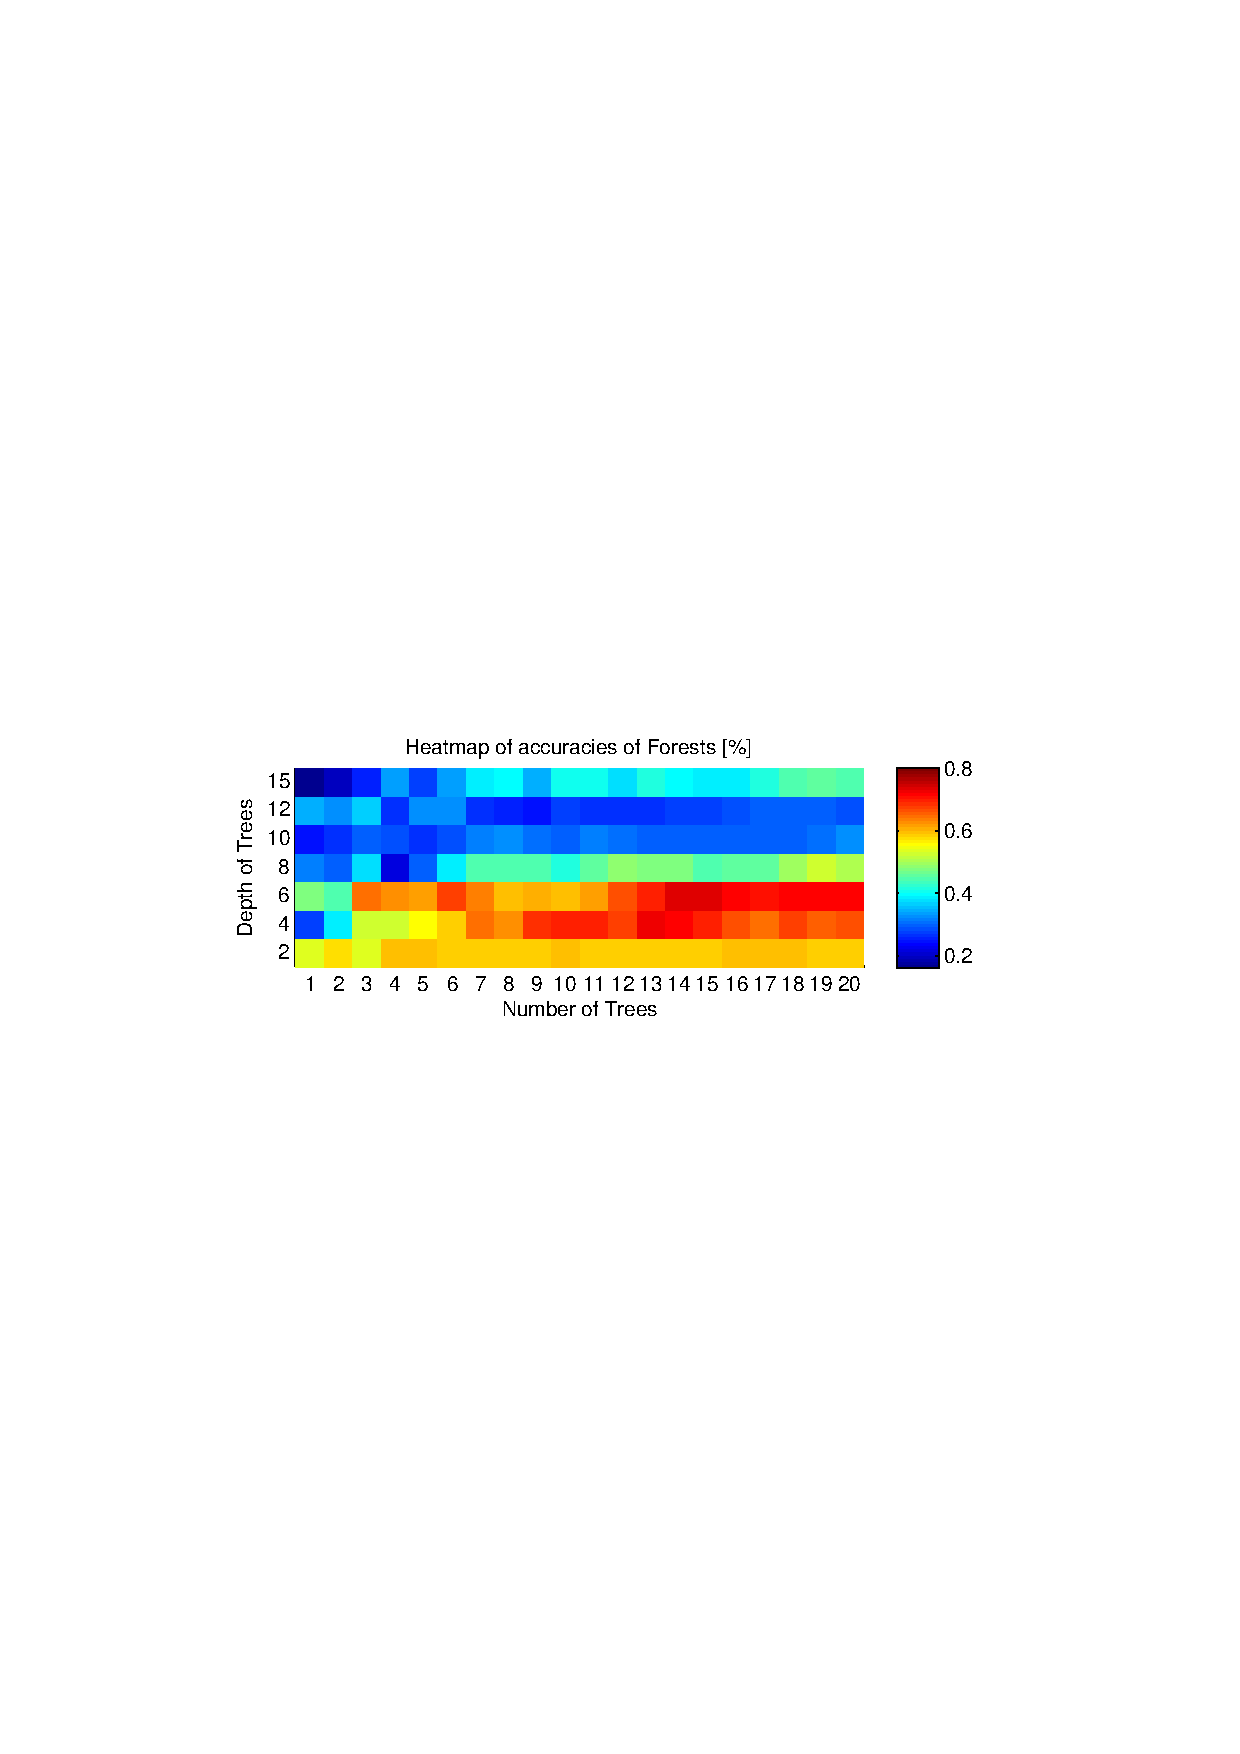
\includegraphics[width=\textwidth]{Diagrams/Forests_Heatmap_Gini_15_20}
\caption{Accuracies of a Forest depending on its number of Trees and the depth of its\\\phantom{Figure 1: }Trees.}
\label{forest_heatmap}
\end{figure}
\begin{figure}[t] 
\centering
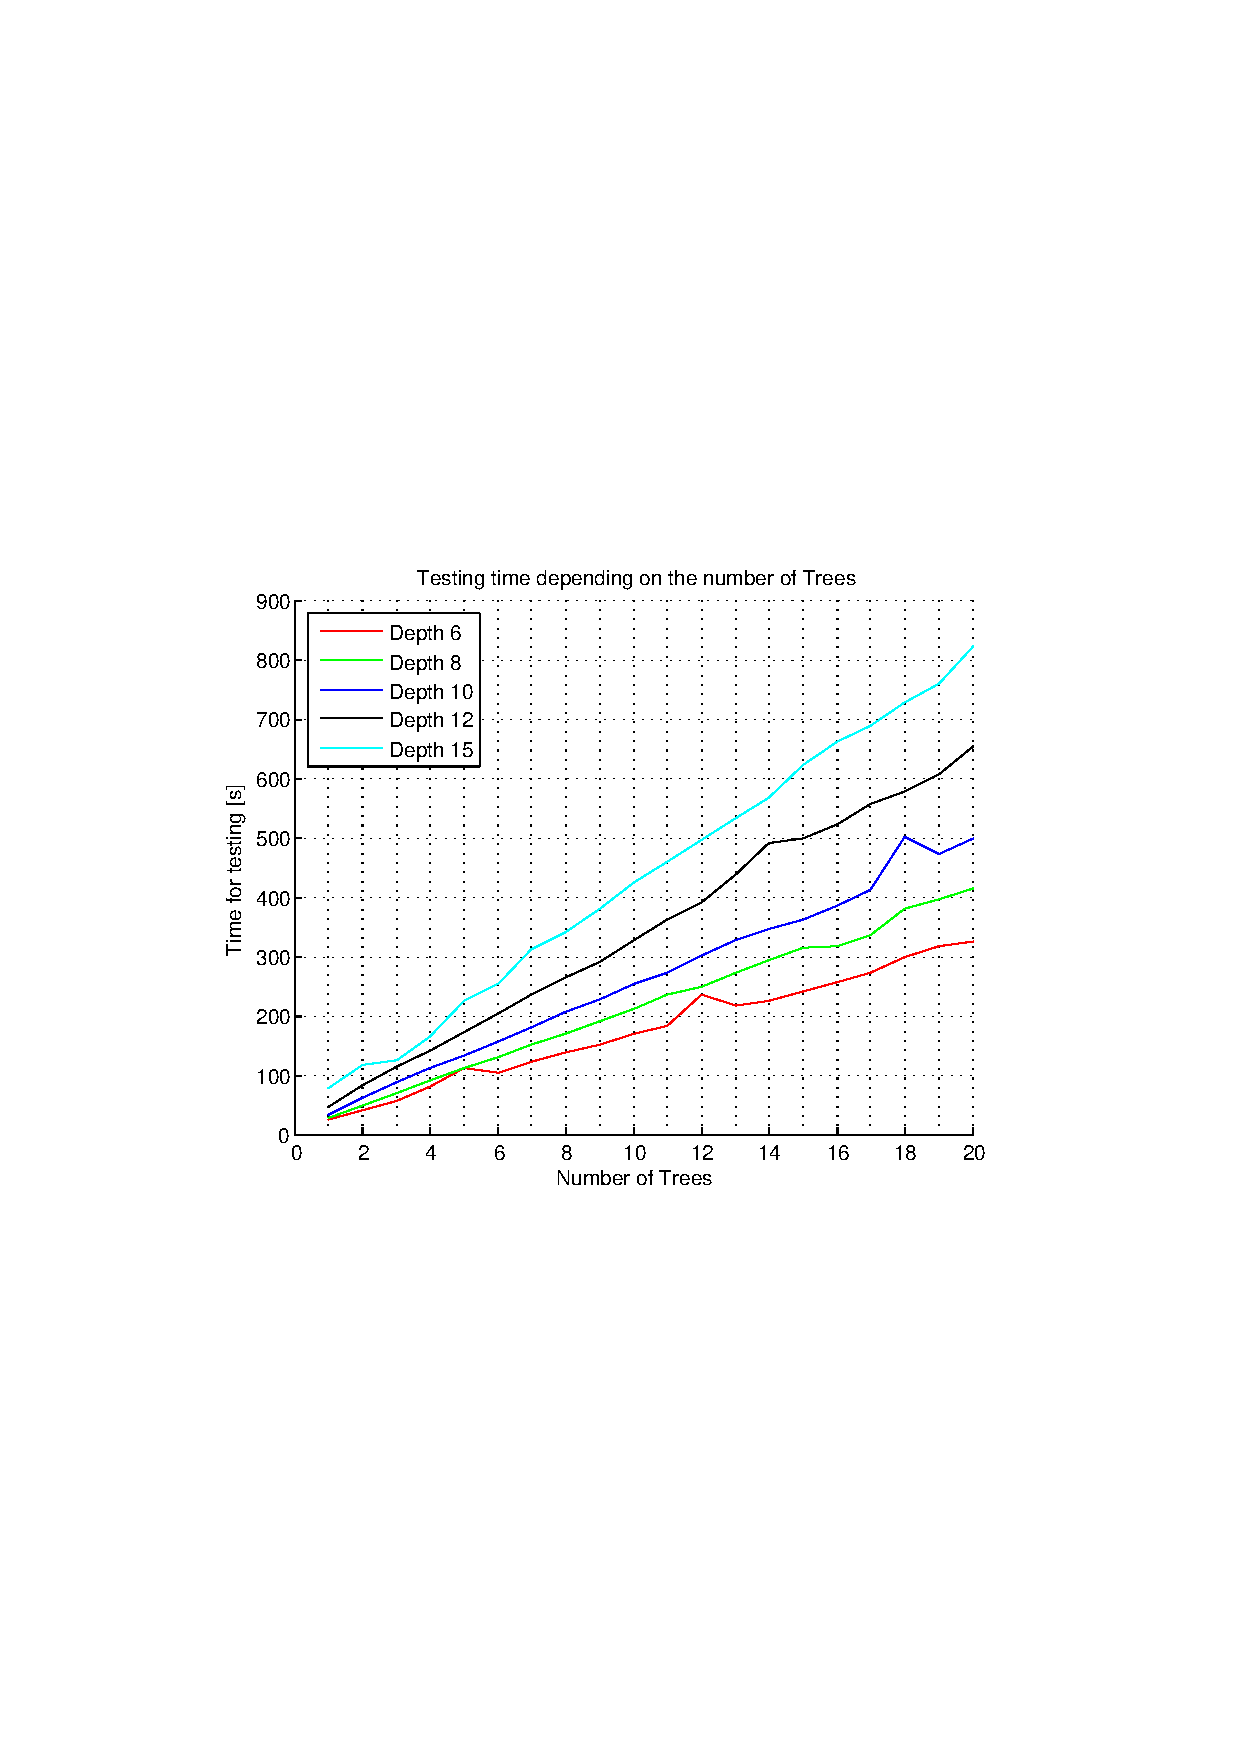
\includegraphics{Diagrams/Forests_Testing_Times_Gini_15_20}
\caption{Testing time of a Forest on the whole testing data set depending on its number\\\phantom{Figure 2: }of Trees. The data was evaluated for five different depths of the Trees of a Forest.}
\label{forest_testing_time}
\end{figure}
\twocolumn





\subsection{Ferest}

\subsubsection{Random Ferest}

First, we tested the original implementation of Ferests which is very fast to train and still very accurate even for its random tests on random features:

It is recognizable that the accuracy of a Ferest tends to increase with increasing number of Ferns and their depths (see Figure \ref{ferest_heatmap}). In Figure \ref{ferest_accuracies} one can see that there is a limit for the best accuracy a Ferest with Ferns of a certain depth can reach - even for up to a hundred Ferns, the best result that could be achieved on the given setup for our data set was around 88\%. This means that a Ferest stops improving once it reaches its maximum accuracy but rather than giving worse results it reaches a plateau and stays there. The largest improvements for this implementation were found within the range of the first ten Ferns in a Ferest.\\
Also, in Figure \ref{ferest_accuracies} the influence of chance can be seen when looking at the plots for depths one and two. Due to the choice of a random threshold, it is possible to choose a bad value or feature. This leads to the depicted unsteady behaviour - especially for Ferests with low depths this effect is quite strong. The same characteristic can be seen in Figure \ref{ferest_heatmap}, e.g. for depth 6 and 25 Ferns in the structure. This effect seems to dissolve the deeper a Fern becomes.

Nevertheless, the depth of a Fern can also become critical when chosen too large. Where Trees tend to overfit for such settings, the number of buckets for the histograms of a Fern increases dramatically. Accordingly, very few samples drop into each bucket while training and therefore, the class-conditional probability distribution is close to being uniform. Informally, every Fern is then uncertain to which class a new sample might belong.\\
This shows that when increasing the depth of a Ferest, the number of samples in the training set should increase exponentially - for our chosen training set, the best depth seems to be ten.

\begin{figure}[h] 
\centering
\includegraphics[width=0.49\textwidth]{Diagrams/heatmap_randFerns_16_30}
\caption{Heatmap for accuracies of a Ferest with different depths and numbers of Ferns}
\label{ferest_heatmap}
\end{figure}

Due to restrictions in time and computation power, we could neither further increase the depth of the used Ferns nor the number of Ferns. But for single samples the following assumptions were confirmed: 
\begin{itemize}
\item After reaching a certain depth, a tendency of decreasing accuracies occurs
\item For depths that are higher than a certain threshold, classification accuracy steadily increases for larger Fern-numbers until it stagnates at a certain value
\end{itemize} 

\begin{figure}[h] 
\centering
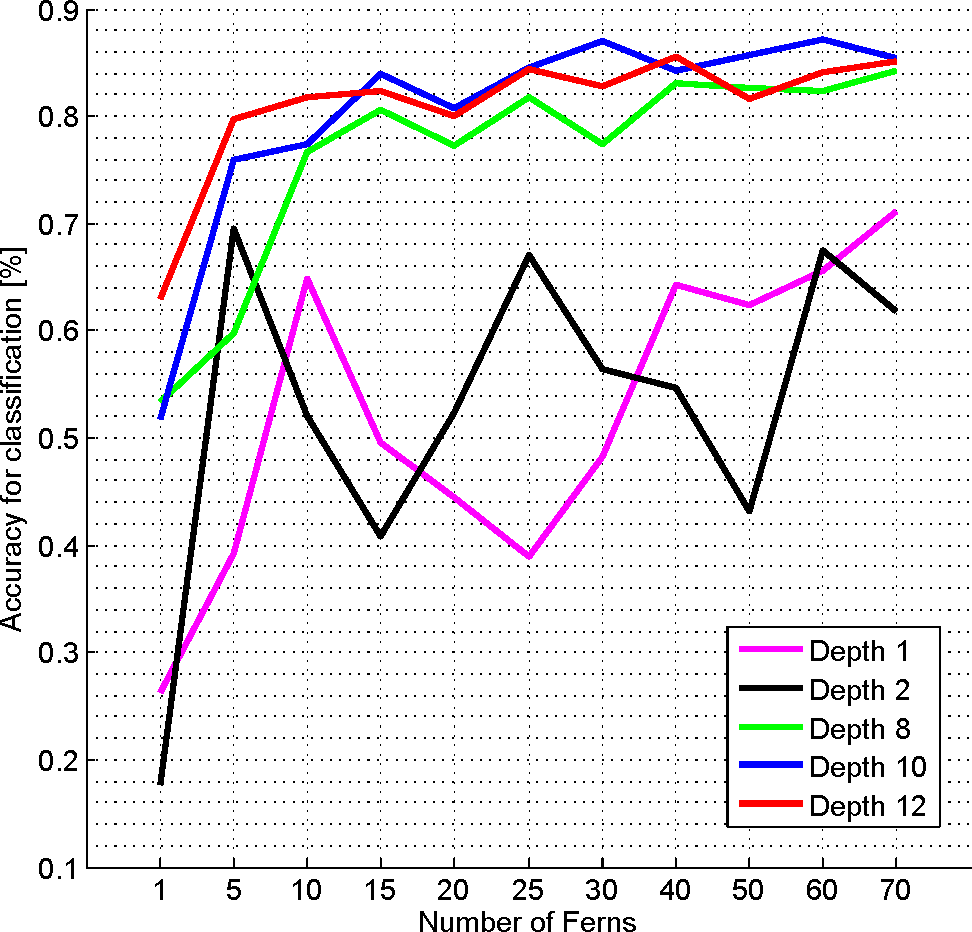
\includegraphics[width=0.49\textwidth]{Diagrams/accuracies_RandFerns_12_70}
\caption{Accuracies of a Ferest for large numbers of Ferns}
\label{ferest_accuracies}
\end{figure}

\subsubsection{Optimized Implementations}

Additionally to the original 'completely' random version of the Ferest, we implemented \textit{bestGini} and \textit{meanRandom}. But where training of a single Fern of the same depth took only 15 seconds for 'random' implementations, it already lasted 20 minutes for the heuristical option incorporating costs with Gini as impurity measure. Nevertheless, \textit{bestGini} was still faster for the training by orders of magnitude (see next section about Comparison).

\begin{tabular}{p{3cm}|p{3cm}|p{5cm}|p{5cm}|p{5cm}}
Depth & #Ferns & \textit{random} & \textit{meanRandom} & \textit{bestGini}\\
8 	& 1 	& 0 	& 66.26\% 	& 73.25\% \\
\end{tabular}

\subsection{Comparison}


\onecolumn
\section*{References}

\begin{tabular}{p{1cm}p{11cm}}

$[1]$ & M. \"Ozuysal, P. Fua, and V. Lepetit. Fast Keypoint Recognition in Ten Lines of Code. \textit{2007 IEEE Conference on Computer Vision and Pattern Recognition}, pages 1-8, June 2007\\
 & \\
$[2]$ & M. B. Kursa. Random ferns method implementation for the general-purpose machine learning. \textit{Interdisciplinary Centre for Mathematical and Computational Modelling, University of Warsaw}, February 2012

\end{tabular}



\end{document}
